\subsubsection{Sistema de control PID}
Un controlador PID (Proporcional-Integral-Derivativo) es un tipo de controlador utilizado en sistemas de control automático para mantener una variable de algún proceso lo más cercana posible a un valor deseado, conocido como "setpoint", a pesar de las perturbaciones encontradas. La acción proporcional responde al error actual, que es la diferencia entre el valor deseado y el valor medido, ajustando la salida del controlador proporcionalmente a este error. Por otro lado, la acción integral se enfoca en la acumulación de errores pasados para eliminar cualquier error que sea persistente, asegurando que con el tiempo la variable de proceso converja al setpoint establecido. Finalmente, la acción derivativa considera la tasa de cambio del error, anticipando y corrigiendo cualquier futura tendencia del error, sumando a la estabilidad del sistema.

El objetivo principal de un controlador PID es proporcionar una respuesta rápida y estable en diferentes aplicaciones. Además de ser utilizado en procesos industriales como plantas químicas y refinerías, también se lo utiliza en el control de velocidad de motores eléctricos, asegurando que el motor funcione a la velocidad deseada sin fluctuaciones por mas que se perciban alteraciones, por lo que en robótica resultan útiles para el control de posición y movimiento, permitiendo acciones precisas y controladas.

\paragraph{Función de transferencia del motor} \mbox{} \vspace{8pt} \\
La función de transferencia en un sistema de control se representa como $G(s)$ y modela matemáticamente el comportamiento de un actuador, al cual se le aplica un estimulo o señal $R(s)$ y se obtiene una respuesta $C(s)$ por parte de él.

Para controlar la variable en cuestión debemos tener una noción sobre la salida producida. Por un lado tenemos la función $H(s)$, que es una función que toma como entrada una medición sobre la salida del actuador o sistema para producir un valor $B(s)$. Éste se suma negativamente al setpoint $R(s)$ para obtener el error entre ellas $E(s)$, que es la señal efectivamente que se introduce a $G(s)$ para logar aproximarse al setpoint y compensar el sistema.

\begin{figure}[H]
    \centering
    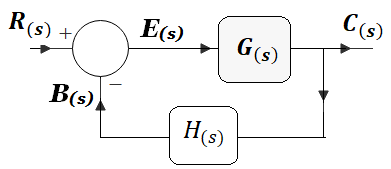
\includegraphics[width=0.4\linewidth]{sistema_de_control}
    \caption{Sistema de control realimentado}
    \label{fig:sistcontrolrealim}
\end{figure}

Para lograr controlar cada motor de cada rueda es necesario conocer la función de transferencia del mismo para lograr modelarlo. Al no contar con la hoja de datos del fabricante por ser un motor genérico, se realizaron una serie de experimentos para aproximar la función $G(s)$. En nuestro caso debemos obtener una función de transferencia que tenga como entrada $[Volts]$ y su salida sea $[RPM]$.

Para hacer esto se propone hacer uso del método de la constante de tiempo $\tau$. En primer lugar, consideraremos que la curva alcanza el $63.2\%$  del valor final cuando ha transcurrido un tiempo $t=\tau$. En la gráfica el valor final de la curva es 1, es decir, $y(\infty)=1$. Por lo que debemos identificar el instante $t$ para el cual se cumple que $y(t)=0.632$.

El paso siguiente es trazar una recta paralela al eje de las abscisas (eje $t$) que corresponda al $63.2\%$ del valor final de $y(t)$. Desde ese punto, se traza una recta paralela al eje de las ordenadas (eje $y$) hasta cortar el eje $t$. Este punto de intersección corresponde al valor de $\tau$.

\begin{figure}[H]
    \centering
    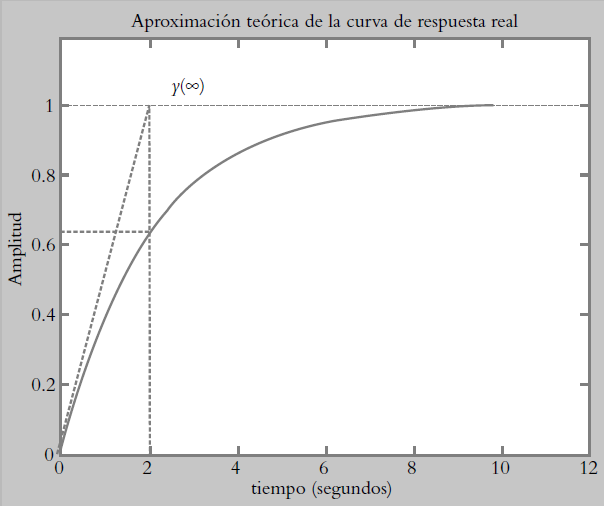
\includegraphics[width=0.625\linewidth]{metodo_const_tiempo_func_transf}
    \caption{Método de la constante de tiempo}
    \label{fig:metodoctetiempo}
\end{figure}

Obtenido esto, se procede a elaborar un sistema de primer orden mediante la siguiente expresión:

$$ G(s) = \frac{k}{\tau \cdot s + 1} $$

Donde $k$ representa la ganancia estática, que es el valor al que tiende la salida del sistema cuando la entrada es una señal constante y el tiempo tiende a infinito. En otras palabras, es el factor de escala entre la entrada y la salida en estado estacionario.

Para identificar la ganancia estática $k$, partimos de que en estado estacionario la salida alcanza un valor constante $y(\infty)$. Además, se considera que estimulamos al actuador con una señal escalón, denominada $u(\infty)$. La ganancia estática se puede calcular como:

$$ k=\frac{y(\infty)}{u(\infty)} $$

Para medir la respuesta del motor, primero conectamos mecánicamente el eje del motorreductor a medir junto con el eje de otro motor testigo, el cual esta conectado a un osciloscopio. Con esta experiencia buscamos estimular al motorreductor con una señal escalón unitario y que el motor testigo genere una tensión que se puede registrar en el osciloscopio. De este modo obtuvimos los valores de tensión generada en el motor testigo y podemos estimar la respuesta del motorreductor. En la Figura \ref{fig:exprespmotor} se muestra un diagrama de la experiencia.

\begin{figure}[H]
    \centering
    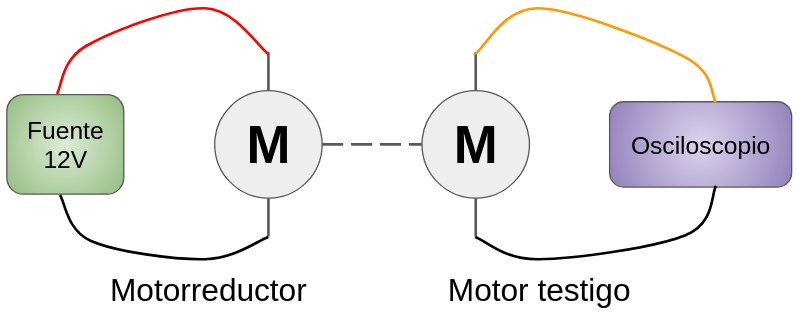
\includegraphics[width=0.55\linewidth]{experim_resp_motor}
    \caption{Experiencia para medición de RPM}
    \label{fig:exprespmotor}
\end{figure}

En el osciloscopio logramos obtener la gráfica que se muestra en la Figura \ref{fig:curvarespmotor}. En amarillo se representa la entrada escalón de 12V hacia el motor y en verde la tensión generada en el motor testigo.

\begin{figure}[H]
    \centering
    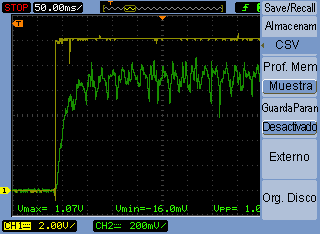
\includegraphics[width=0.525\linewidth]{curva_resp_motor_osciloscopio}
    \caption{Curva de respuesta del motorreductor}
    \label{fig:curvarespmotor}
\end{figure}

Luego procedimos a extraer los puntos de datos y suavizar la curva para facilitar el análisis. Esto lo hicimos mediante una media ponderada con un factor $\alpha = 0.2$, obtenido experimentalmente:

$$ S_{t} = \alpha \cdot Y_{t-1} + (1 - \alpha) \cdot Y_{t} $$

A partir de ello obtuvimos la gráfica de la Figura \ref{fig:curvarespmotorsuaviz}, donde en el eje horizontal están representados instantes de tiempo equivalentes a $10[ms]$ cada uno y en el eje vertical el voltaje (expresado en $[volts]$) sensado en el motor testigo.

Ahora bien, para linealizar el sistema podemos suponer que el valor de tensión generado en el motor testigo es proporcional a las revoluciones por minuto que gira su eje. Dado que en la iteración anterior se logró la implementación de un medidor de RPM, obtuvimos en este caso que el motorreductor conectado a 12V continuos produce 92 [RPM]. En este momento podemos calcular la ganancia estática $k$:

$$ k=\frac{y(\infty)}{u(\infty)}=\frac{92[RPM]}{12[V]}=7.66[RPM/V] $$

\begin{figure}[H]
    \centering
    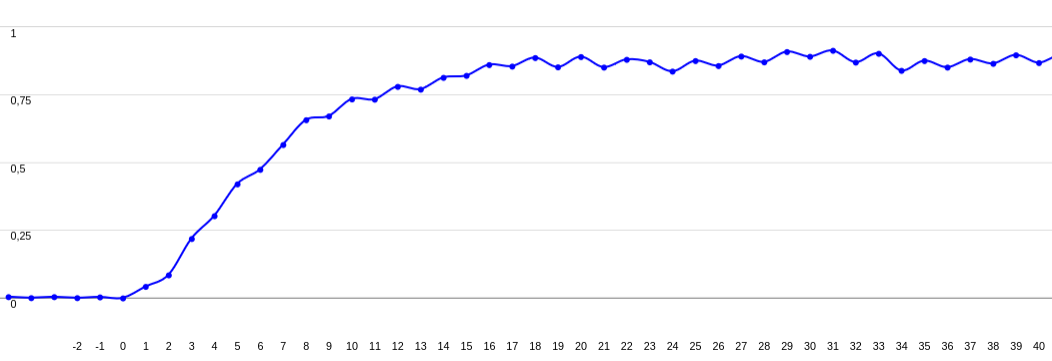
\includegraphics[width=1.0\linewidth]{resp_motor_suavizado}
    \caption{Curva de respuesta del motor suavizada}
    \label{fig:curvarespmotorsuaviz}
\end{figure}

Por otra parte, determinamos que $\tau=70[ms]$ por alcanzar en esa marca el valor de tensión $0,564[V]$, rondando el $63.2\%$ del valor en estado estacionario. Aplicando la expresión para obtener un sistema de primer orden obtenemos:

$$ G(s) = \frac{7.66}{0.07 \cdot s + 1} $$

% https://dademuchconnection.wordpress.com/2021/06/26/aproximacion-teorica-de-una-curva-de-respuesta-real/
% https://controlautomaticoeducacion.com/control-realimentado/ziegler-nichols-sintonia-de-control-pid/

\paragraph{Diseño del controlador} \mbox{} \vspace{8pt}

Es tarea del controlador intervenir para corregir las fluctuaciones que sufre el sistema. Por lo general los controladores PID basan su funcionamiento en 3 parámetros fundamentales, los cuales son $K_p$, $K_i$ y $K_d$; correspondiéndose con el factor de acción proporcional, integrativa y derivativa, respectivamente.

En nuestro caso, optamos por utilizar un PID aditivo por ser de sencilla implementación y por ser mas rápida la convergencia a los coeficientes óptimos. En la Figura \ref{fig:pidaditivo} se muestra un diagrama del mismo.

\begin{figure}[H]
    \centering
    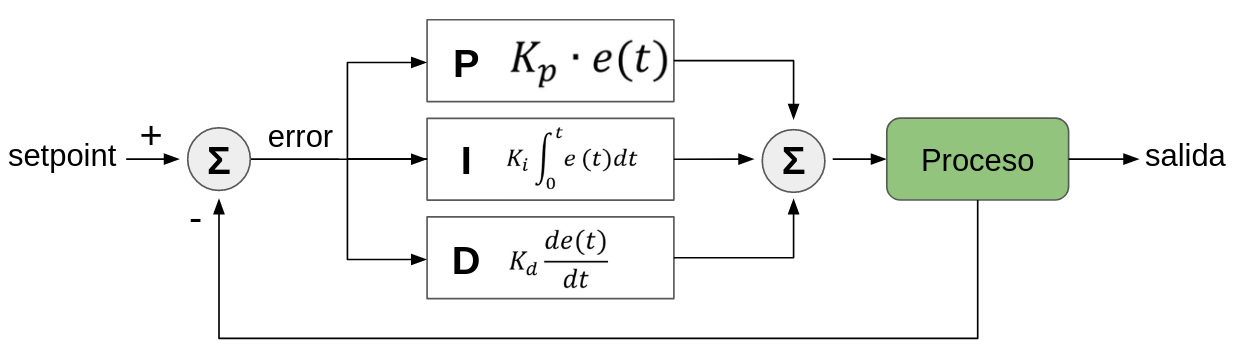
\includegraphics[width=0.9\linewidth]{images/pid_aditivo}
    \caption{PID aditivo}
    \label{fig:pidaditivo}
\end{figure}

\paragraph{Implementación} \mbox{} \vspace{8pt}

Cada uno de los cuatro motores del robot tiene su propio controlador PID, todos con coeficientes idénticos. Se implementan dentro del microcontrolador ESP32 haciendo uso de los puertos de salida PWM para controlar la velocidad y sentido de cada una de las ruedas. Además se utilizan los módulos contadores de pulsos asociados a los puertos GPIO donde se conecta cada encoder rotativo.

Como requerimiento, debe contar con tiempos de respuesta aceptables para que el sistema de control funcione adecuadamente, por lo que hicimos pruebas para descubrir el mejor $\Delta T$ de actualización del PID, en concordancia con el período de medición de RPM. Pudimos determinar que el controlador cumple con el requerimiento teniendo un periodo mínimo de $T=100[ms]$.

Por cada motor se tiene una estructura como la siguiente:

\begin{figure}[H]
    \centering
    \hspace*{-0.75cm}
    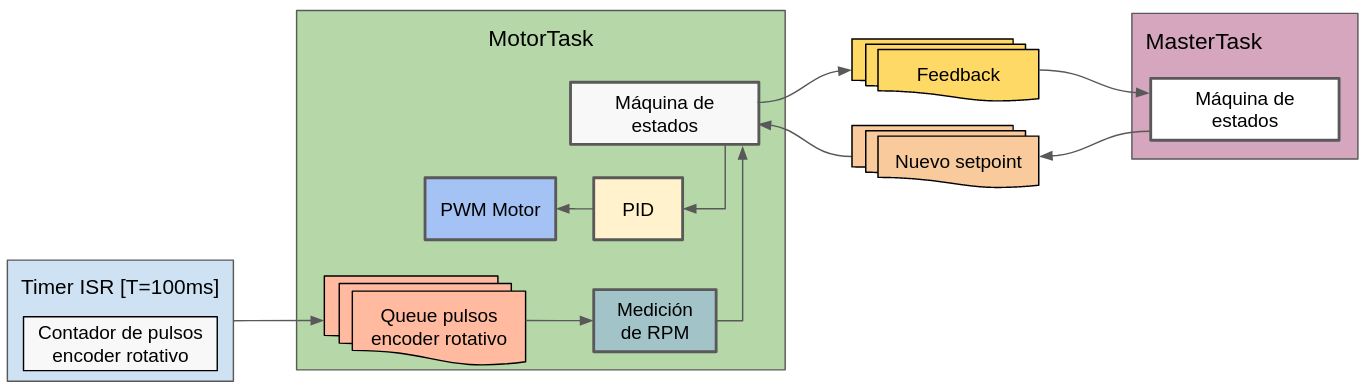
\includegraphics[width=1.1\linewidth]{images/diag_comp_esp32_pid_solo.png}
    \caption{Diagrama de componentes del firmware de la ESP32}
    \label{fig:diagcomponentesp32}
\end{figure}

En primer lugar, se tiene una interrupción periódica de $T=100[ms]$ donde se toman los valores de cada uno de los módulos contadores de pulso (PCNT) del microcontrolador, vinculados a los encoders rotativos de cada rueda. Existe una cola por cada MotorTask para recibir esta información desde la interrupción.

Por otro lado, la tarea MasterTask cuenta con una cola (queue) única que comparte con todas las MotorTask para recibir el feedback de las mismas. Además, cada tarea MotorTask tiene una cola que comparte con la tarea MasterTask, donde se envía un setpoint independiente a cada rueda.

Al ser el robot omnidireccional, si se establecen todas las ruedas a la misma velocidad y en sentidos determinados, es posible lograr que el robot de mueva a lo largo de un vector en linea recta sobre el plano. De este modo podemos llevar a cabo pruebas con las que encontramos los coeficientes del controlador.

A continuación, incurrimos en la utilización de la técnica de Ziegler-Nichols a lazo abierto y logramos obtener valores aproximados de $K_p$, $K_i$ y $K_d$. Introdujimos estos valores en el controlador y colocamos el robot en el suelo para realizar una serie de pruebas en línea recta. Con estos coeficientes no notamos un comportamiento óptimo, por lo que nos enfocamos en iterar sobre los valores y ajustar las constantes.

De este modo se realizaron iteraciones aumentando o disminuyendo cada uno de los coeficientes para buscar el punto óptimo de funcionamiento. Comenzamos con un valor de $K_p=10$ y un setpoint de $65[RPM]$, los demás coeficientes en cero. De este modo se fue aproximando el valor hasta lograr un arranque rápido pero sin demasiado sobrepaso. Una vez obtenido lo anterior, se procedió a ajustar $K_i$ observando cómo variaba el error acumulado al alcanzar las RPM deseadas. Finalmente se determinó el factor $K_d$ mediante observación de la respuesta del robot ante picos de perturbaciones.

Finalmente, obtenemos la siguiente estructura para el control de las 4 ruedas independientes del robot:

\begin{figure}[H]
    \centering
    \hspace*{-0.75cm}
    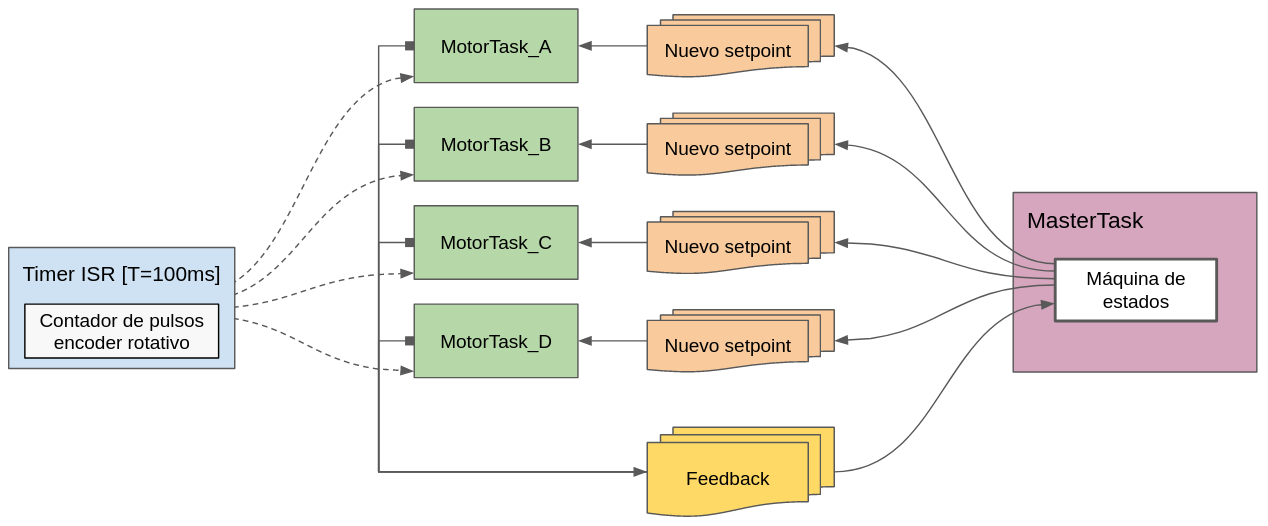
\includegraphics[width=1.1\linewidth]{images/diag_comp_esp32_pid_solo_todos_los_motores.png}
    \caption{Estructura de control de los motores}
    \label{fig:diagcommpesp32pidmotores}
\end{figure}

A continuación se detalla el funcionamiento de una de las tareas de los motores con la tarea principal. El proceso es similar para las demás MotorTask.

\begin{figure}[H]
    \centering
    \hspace*{-1.1cm}
    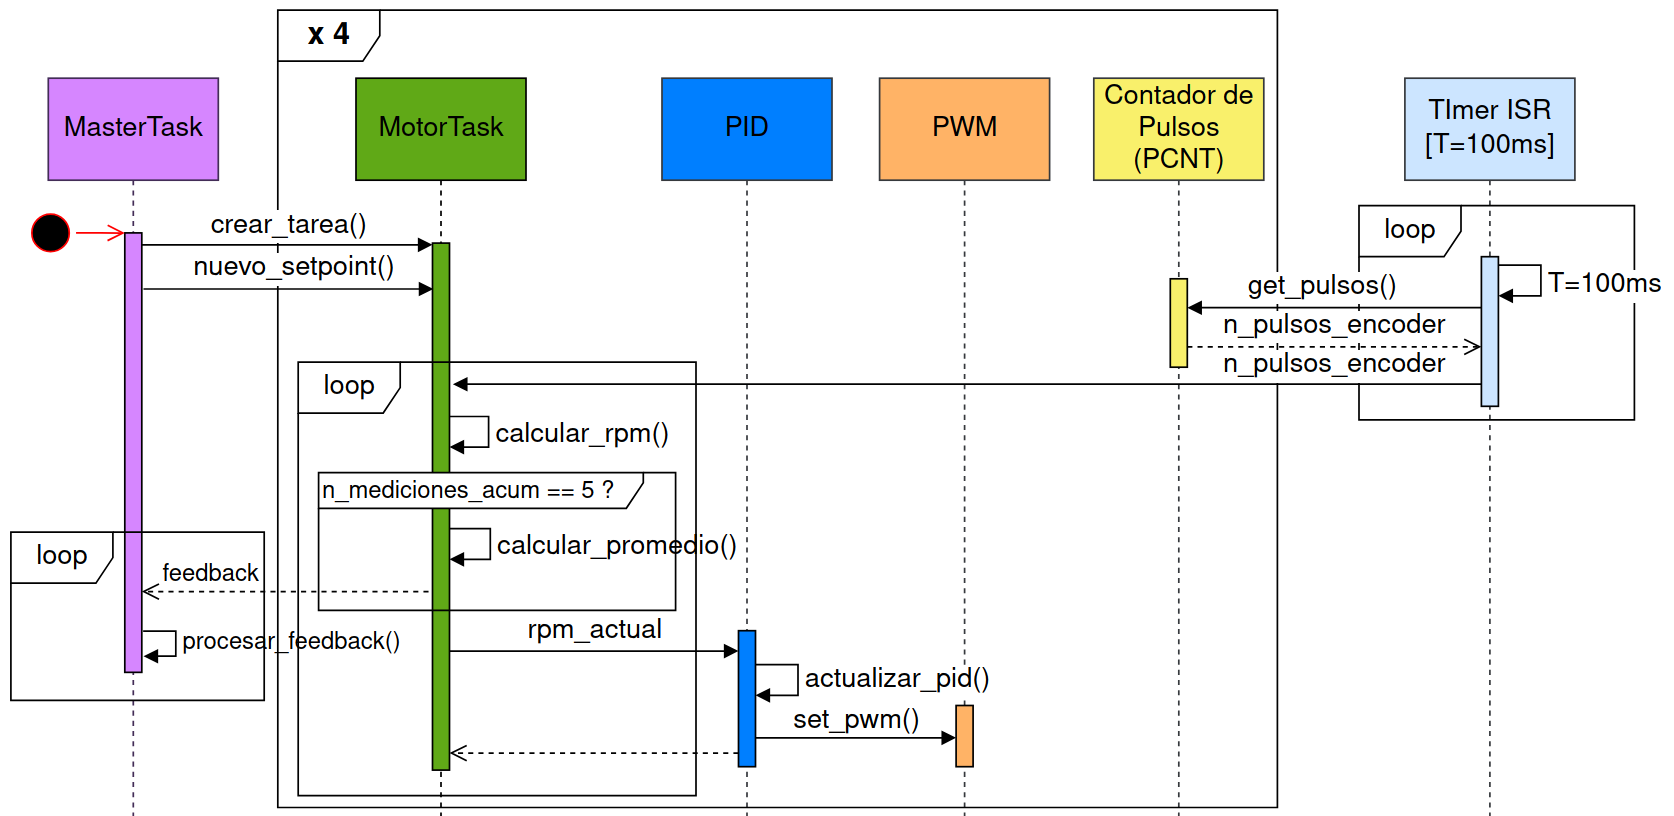
\includegraphics[width=1.15\linewidth]{images/diag_secuencia_pid_solo.png}
    \caption{Diagrama de secuencia de las tareas de control para los motores}
    \label{fig:diagsecuenciapidsolo}
\end{figure}
